\documentclass[noauthor]{ximera}
%handout:  for handout version with no solutions or instructor notes
%handout,instructornotes:  for instructor version with just problems and notes, no solutions
%noinstructornotes:  shows only problem and solutions

%% handout
%% space
%% newpage
%% numbers
%% nooutcomes

%I added the commands here so that I would't have to keep looking them up
%\newcommand{\RR}{\mathbb R}
%\renewcommand{\d}{\,d}
%\newcommand{\dd}[2][]{\frac{d #1}{d #2}}
%\renewcommand{\l}{\ell}
%\newcommand{\ddx}{\frac{d}{dx}}
%\everymath{\displaystyle}
%\newcommand{\dfn}{\textbf}
%\newcommand{\eval}[1]{\bigg[ #1 \bigg]}

%\begin{image}
%\includegraphics[trim= 170 420 250 180]{Figure1.pdf}
%\end{image}

%add a ``.'' below when used in a specific directory.

\newcommand{\RR}{\mathbb R}
\renewcommand{\d}{\,d}
\newcommand{\dd}[2][]{\frac{d #1}{d #2}}
\renewcommand{\l}{\ell}
\newcommand{\ddx}{\frac{d}{dx}}
\newcommand{\dfn}{\textbf}
\newcommand{\eval}[1]{\bigg[ #1 \bigg]}


\author{Jim Talamo}

\outcome{Understand terminology associated with ODEs.}
\outcome{Classify ODE as linear or nonlinear.}
\outcome{Determine the order of an ODE.}
\outcome{Verify if a given function is a solution to an ODE.}
\outcome{Verify if a given function is a solution to an IVP.}
\outcome{Find parameters so a function satisfies an ODE/IVP or explain why no such parameters exist.}

\title{Direction Fields}

\begin{document}
\begin{abstract}
\end{abstract}
\maketitle

\vspace{-0.9in}

\section{Group Work}

\begin{problem} 

Consider the direction field below. 

 \begin{figure}[h!]
 \centering
  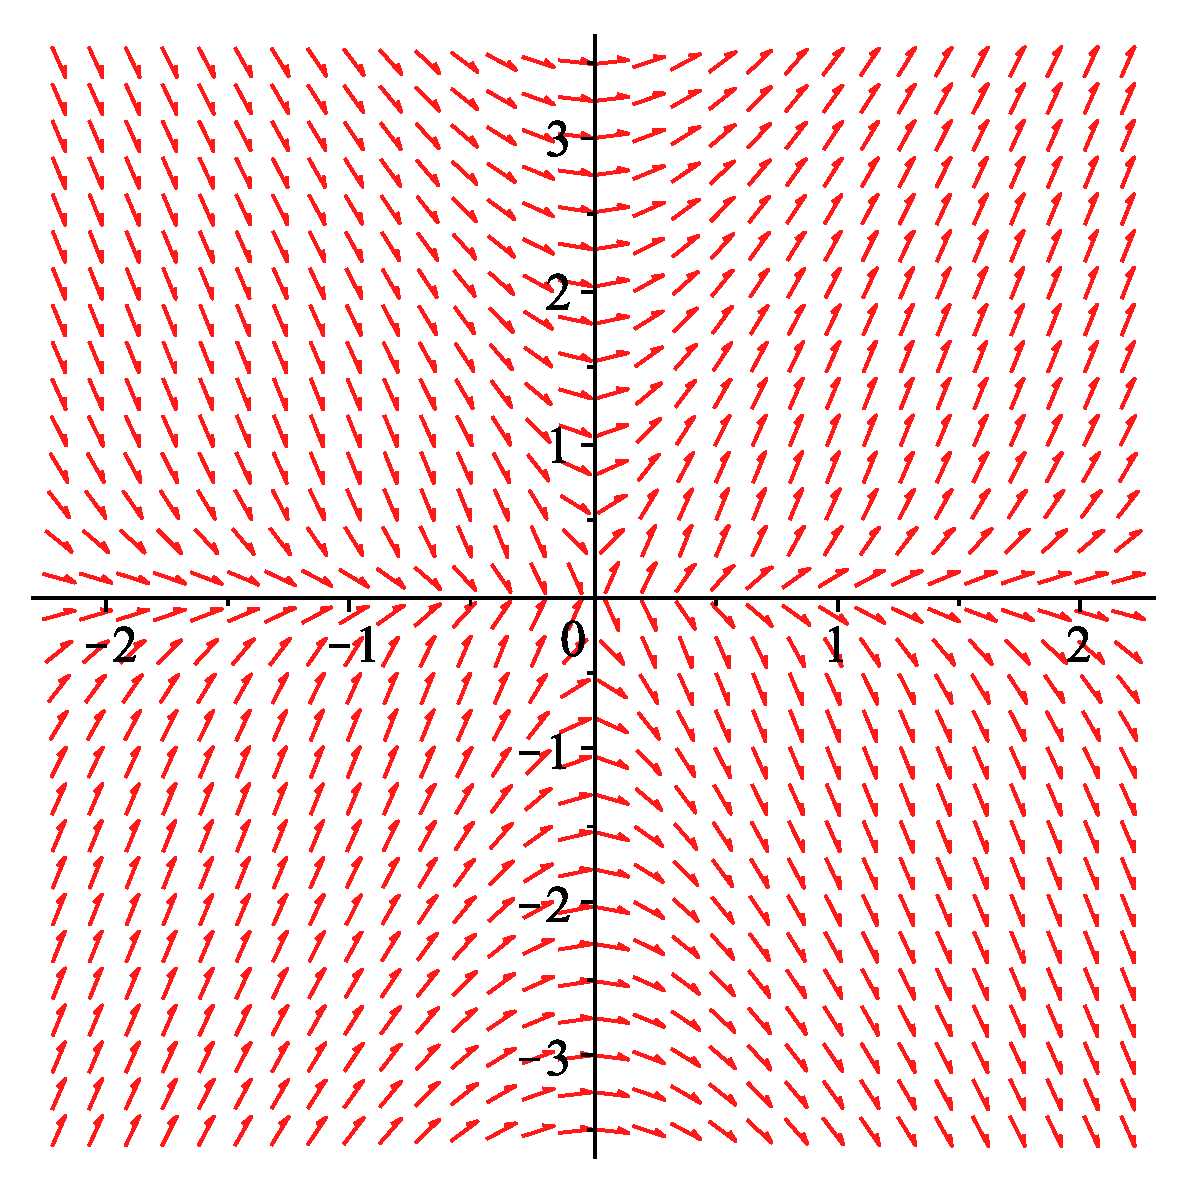
\includegraphics[width=.4 \textwidth]{DirectionField1.eps}
\end{figure}

Which of the following differential equations is represented by this direction field? 

\begin{tabular}{llll}

A. $\dfrac{dy}{dx} = \dfrac{8x^2y}{x^2+y^2}$ \qquad & B. $\dfrac{dy}{dx} = \dfrac{8xy^2}{x^2+y^2}$\qquad & C. $\dfrac{dy}{dx} = \dfrac{8x^2y^2}{x^2+y^2}$\qquad & D. $\dfrac{dy}{dx} = \dfrac{8xy}{x^2+y^2}$ 
\end{tabular}

\begin{freeResponse}
We can rule out functions based on the sign of the slope in each quadrant. Since the slopes are negative in the second quadrant, the functions in A and C are ruled out. Positive slopes in the third quadrant rule out the function in B. This leaves the function in D, and inspection of the slopes shows that they agree with this function.
\end{freeResponse}
\end{problem}
%%%%%%%%%%%%%%%%%%%%
\begin{problem}
The graph of a certain function $y=f(x)$ is shown below.

\begin{center}
\resizebox {5.0cm} {!} { \begin{tikzpicture}
            	\begin{axis}[
            		domain=-2:4, ymax=6.4,xmax=3.4, ymin=-1.4, xmin=-.8,
            		axis lines =center, 
		         xlabel=$x$, 
		         xtick={1,2,3},
		         ylabel=$y$,
		         ytick={1,2,3,4,5,6},
            		every axis y label/.style={at=(current axis.above origin),anchor=south},
            		every axis x label/.style={at=(current axis.right of origin),anchor=west},
            		axis on top,
            		]
                      
            	
            	\addplot [draw=penColor,very thick,smooth] {x^3-4*x^2+4*x+2};		
	 	\node at (axis cs:2.4,5.1) [penColor] {$y=f(x)$};
            	\end{axis}
            \end{tikzpicture}}
\end{center}

Determine whether $y=f(x)$ could be a solution to the initial value problem below and justify your response. 
\[
\dfrac{dy}{dx}-4y=e^{-3x} , \qquad y(0)=2
\]

\begin{freeResponse}
There are many ways see why the given graph will not represent a solution to the IVP.  First, we rewrite the IVP by bringing the differential equation into the form $y'=f(x,y)$.

\[
\dfrac{dy}{dx}=4y+e^{-3x} , \qquad y(0)=2
\]


One observation is that a solution of the IVP must satisfy
$$
\eval{\frac{dy}{dx}}_{x=0} = \eval{4y + e^{-3x}}_{x=0} = 4y(0) + e^0 = 4 \cdot 2 + 1 = 9.
$$
The function graphed above appears to have $f'(0) \approx 3$, so it cannot be a solution of the IVP.

Another observation is that according to the differential equation, $\frac{dy}{dx} >0$ for any $(x,y)$ in Quadrant I, so a solution must be increasing in Quadrant I.  The graph of the function in the image does not satisfy this requirement.
\end{freeResponse}


\end{problem}


%%%%%%%%%%%%%%%%%%%%
\begin{problem} 
Which of the following is the direction field for the differential equation $\dfrac{dy}{dx} = \dfrac{y-2x}{2}$ ?


 \begin{figure}[!htb]
 \hspace{10mm} \minipage{0.4\textwidth} 
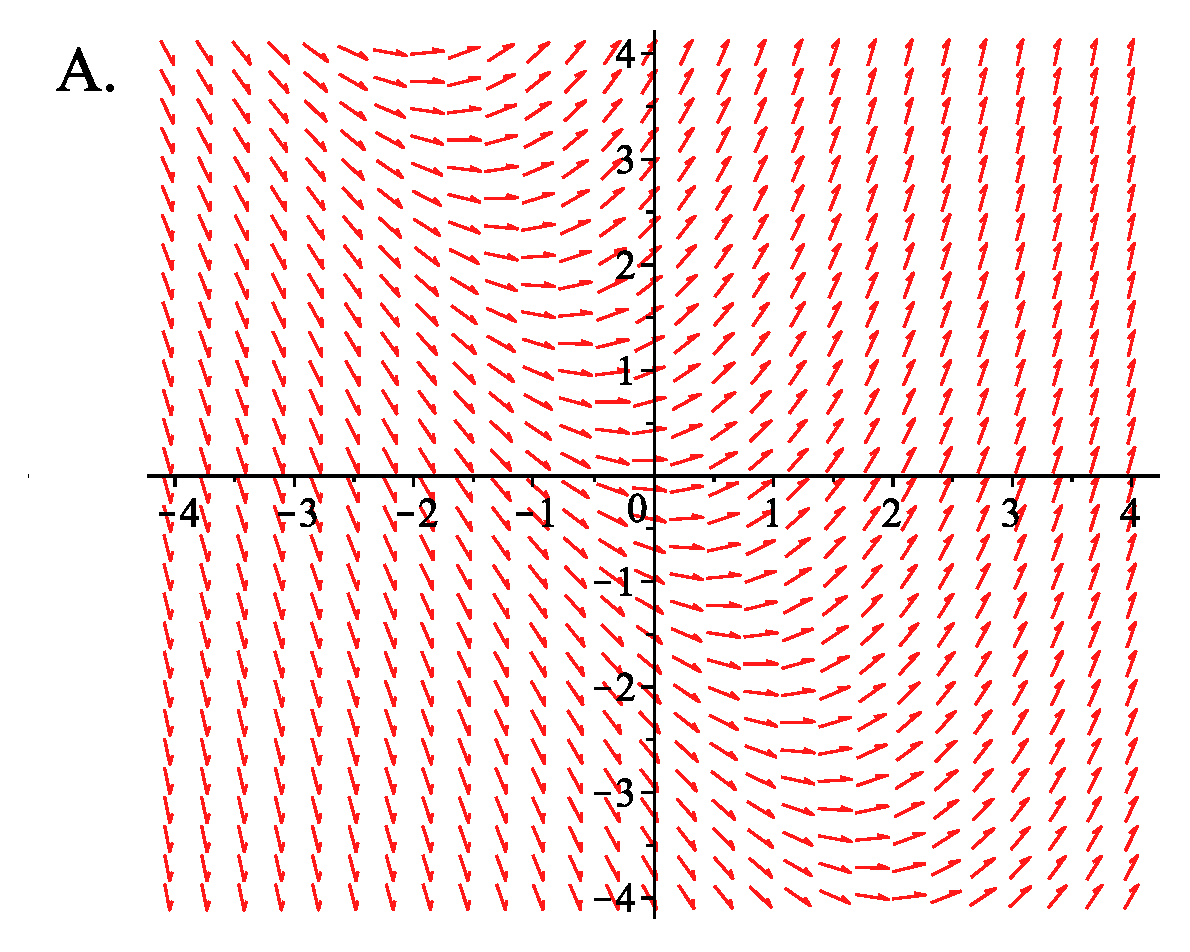
\includegraphics[width=\linewidth]{MCA.eps} 

  \endminipage \hspace{10mm} 
\minipage{0.4\textwidth}%
  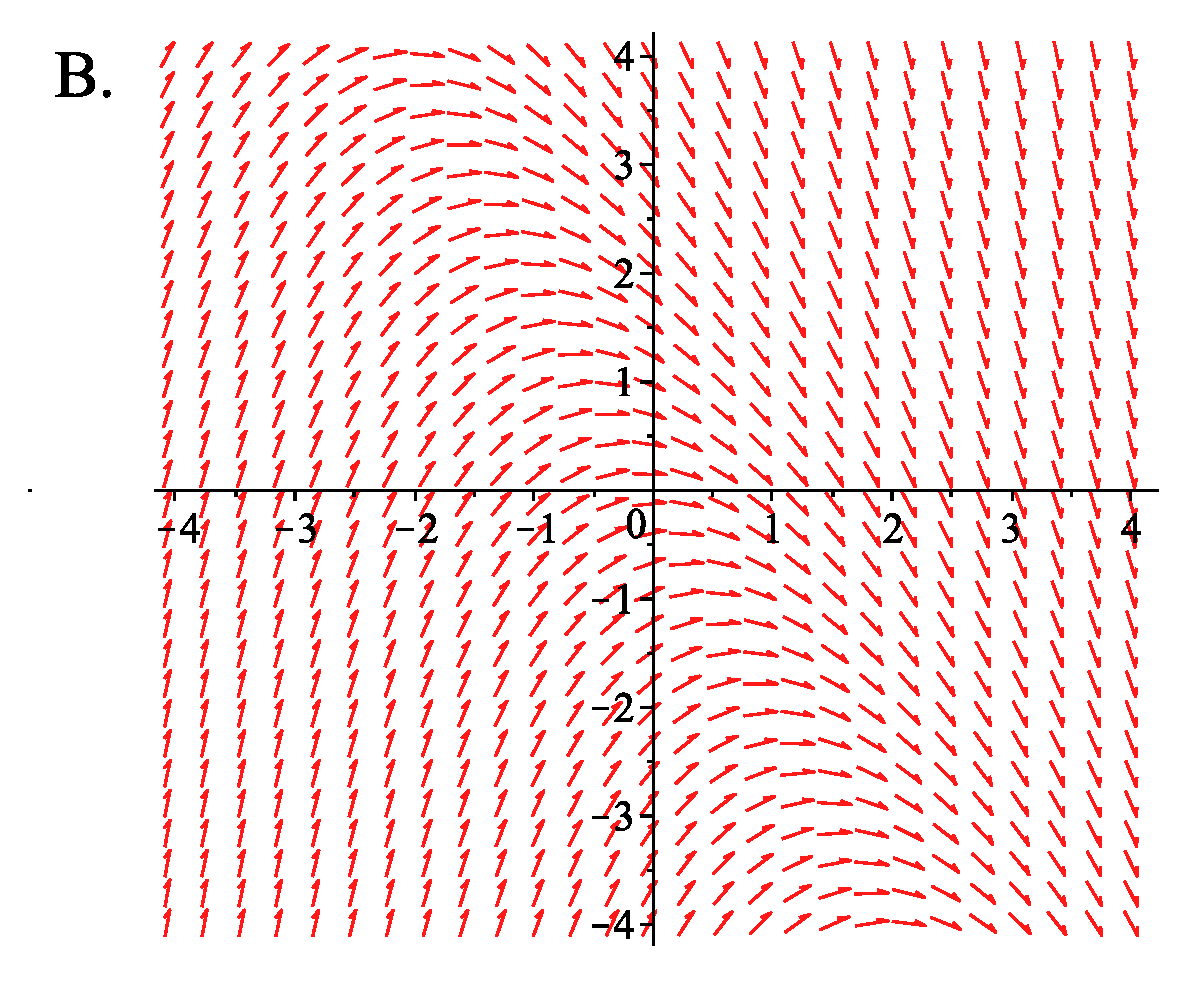
\includegraphics[width=\linewidth]{MCB.eps}

\endminipage

\end{figure}

\begin{figure}[!htb]
\hspace{10mm} \minipage{0.4\textwidth} 
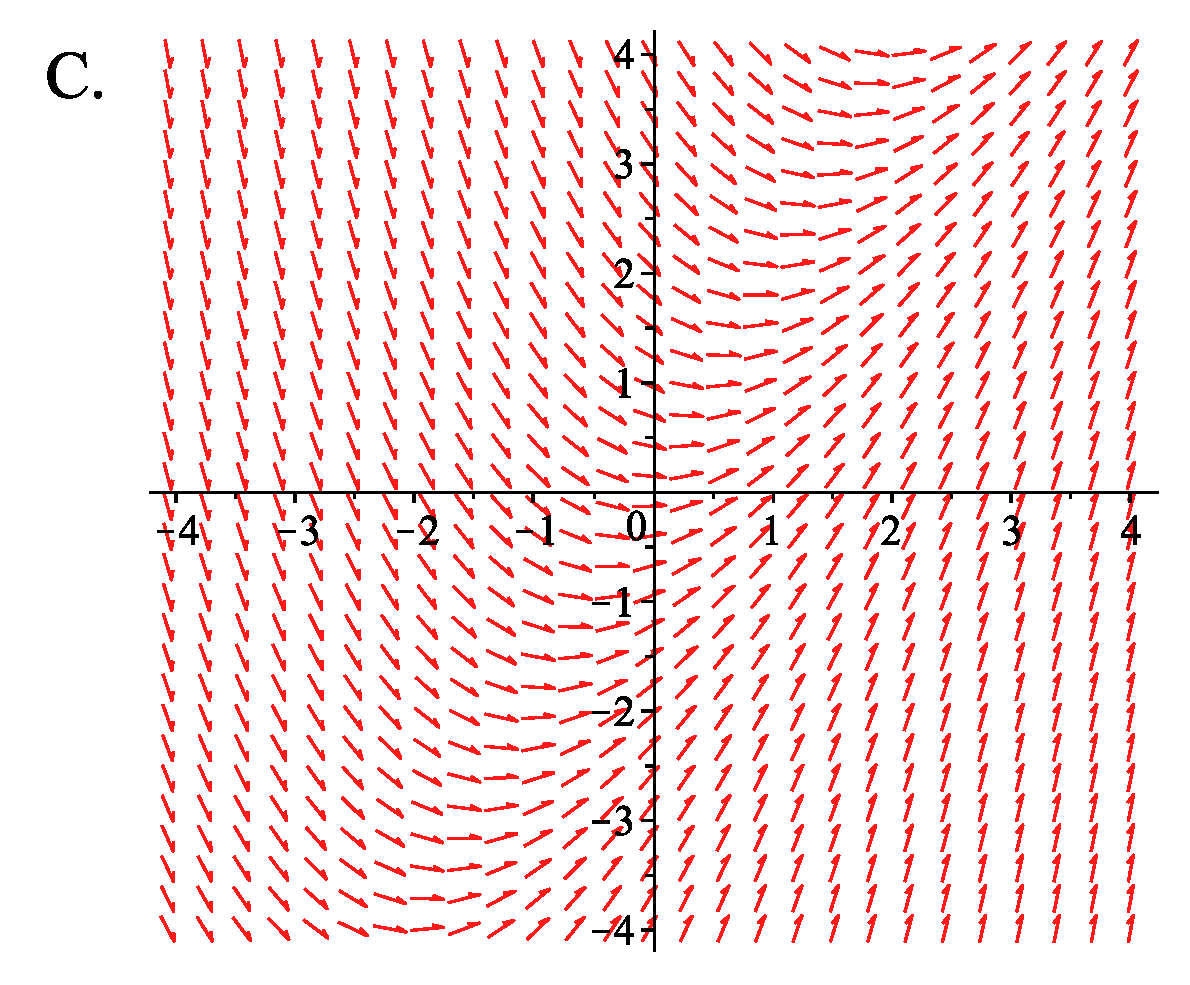
\includegraphics[width=\linewidth]{MCC.eps} 

  \endminipage \hspace{10mm} 
\minipage{0.4\textwidth}%
  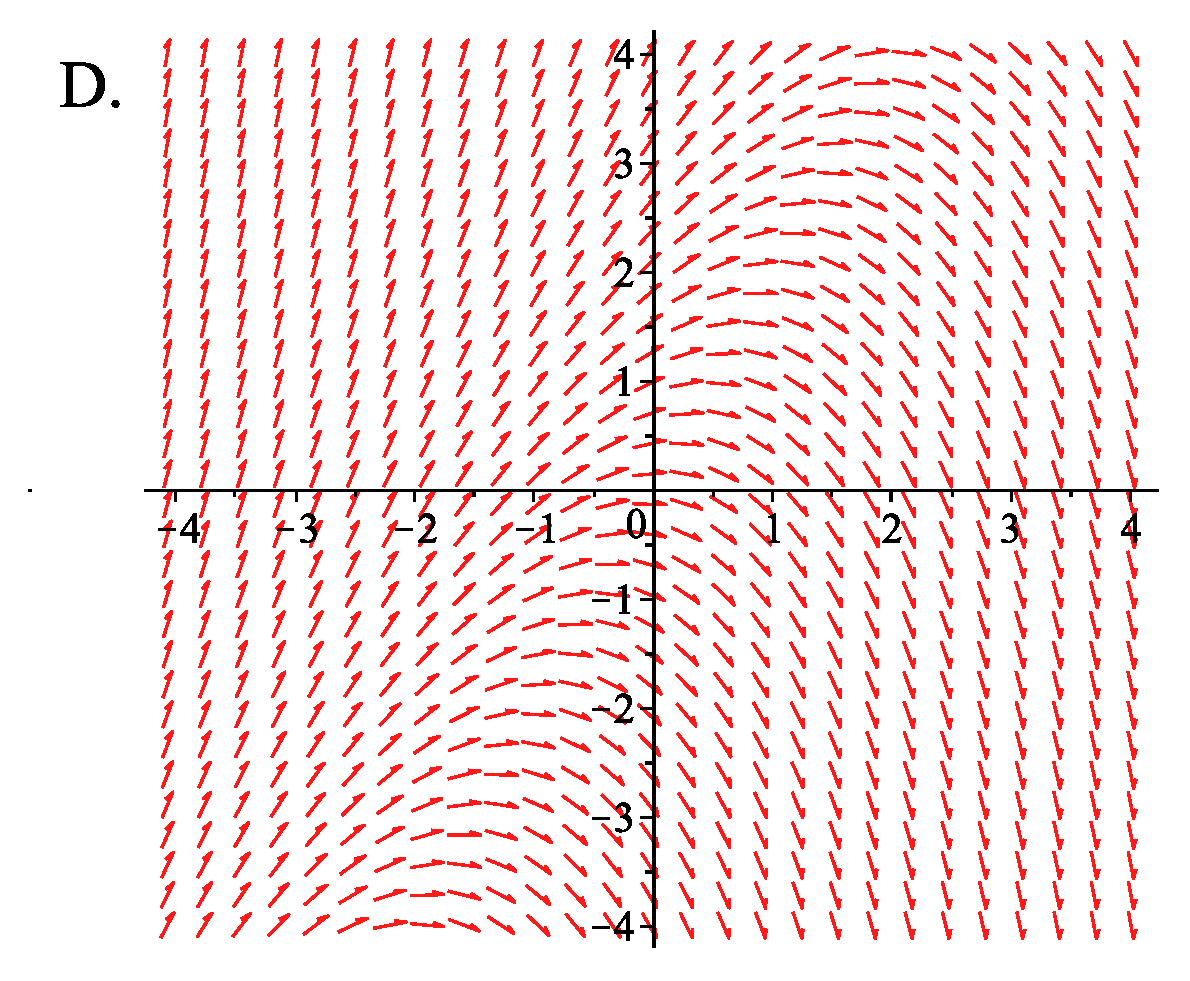
\includegraphics[width=\linewidth]{MCD.eps}

\endminipage

\begin{freeResponse}
First note that $\frac{dy}{dx}=0$ along the line $y=2x$. This rules out the direction fields in A and B, but appears to be the case for the direction fields in C and D. Next note that in the second quadrant, $y > 0$ and $x < 0$ implies that $y-2x > 0$, so that the direction field must have positive slope. Therefore the correct direction field is the one appearing in D.
\end{freeResponse}
\end{figure}


\end{problem}







\end{document}
